\documentclass[a4paper, landscape]{article}

\usepackage[utf8]{inputenc}
\usepackage[DIV=12]{typearea}
\usepackage{microtype}
\usepackage{mathtools, amssymb}
\usepackage{parskip}
\usepackage{graphicx}
\usepackage{subcaption}
\graphicspath{ {./results} }
\usepackage{float}
\usepackage[colorlinks=true]{hyperref}
\hypersetup{linktoc=all}

\title{6}
\date{}

\begin{document}
\maketitle
\section{Ground Truth Images}
Figure \ref{fig:o} displays the ground truth images for each $k$.

The selected DCT columns and their coefficients of an image with a $k$ value are carried forward in the image generation with higher $k$ values.

To generate a different set of images, simply change the value of variable \verb!seed!.

\textbf{Note:} While running \verb!myMainScript!, please do not close the figure window that appears after data generation completion of OMP algorithm.
\begin{figure}[H]
    \centering
    \begin{subfigure}{0.09\linewidth}
        \centering
        
\includegraphics[width=\linewidth]{k = 5.png}
        \caption{$k = 5$}
    \end{subfigure}
    \begin{subfigure}{0.09\linewidth}
        \centering
        
\includegraphics[width=\linewidth]{k = 10.png}
        \caption{$k = 10$}
    \end{subfigure}
    \begin{subfigure}{0.09\linewidth}
        \centering
        
\includegraphics[width=\linewidth]{k = 20.png}
        \caption{$k = 20$}
    \end{subfigure}
    \begin{subfigure}{0.09\linewidth}
        \centering
        
\includegraphics[width=\linewidth]{k = 30.png}
        \caption{$k = 30$}
    \end{subfigure}
    \begin{subfigure}{0.09\linewidth}
        \centering
        
\includegraphics[width=\linewidth]{k = 50.png}
        \caption{$k = 50$}
    \end{subfigure}
    \begin{subfigure}{0.09\linewidth}
        \centering
        
\includegraphics[width=\linewidth]{k = 100.png}
        \caption{$k = 100$}
    \end{subfigure}
    \begin{subfigure}{0.09\linewidth}
        \centering
        
\includegraphics[width=\linewidth]{k = 150.png}
        \caption{$k = 150$}
    \end{subfigure}
    \begin{subfigure}{0.09\linewidth}
        \centering
        
\includegraphics[width=\linewidth]{k = 200.png}
        \caption{$k = 200$}
    \end{subfigure}
    \caption{Original images}
    \label{fig:o}
\end{figure}
\section{Reconstructed Images}
\subsection{Task 1}
For $k \in \{5,10,20,30,50,100,150,200\}$ and $m \in \{100,200,\ldots,1000\}$.

OMP and IHT algorithms are implemented in the \verb!code! directory and the reconstructed images and the RMSE values are located in the \verb!results! directory. RMSE values are stored as a 2-D matrix with row index corresponding to the respective $k$ value index and column index corresponding to the respective $m$ value index.
\subsection{Task 2}
For $k \in \{5,50,200\}$ and $m \in \{100,200,\ldots,1000\}$.

RMSE plots are shown in \ref{fig:ck} and reconstructed images are shown in \ref{fig:ok} and \ref{fig:ik}.

As seen by the plots RMSE values are lesser than 1 for both algorithms implying a good reconstruction. For OMP, they tend to zero very quickly for $k\in\{5,50\}$ whereas the $k=200$ case needed $800$ measurements for RMSE to become very small. For IHT, images are almost same to the actual images in all cases except for $(k,m)\in\{(50,100), (200,100), (200,200), (200,300), (200,400)\}$. Implying that as $k$ increases, more measurements are required for a perfect reconstruction.
\begin{figure}[H]
    \centering
    \begin{subfigure}{0.45\linewidth}
        \centering
        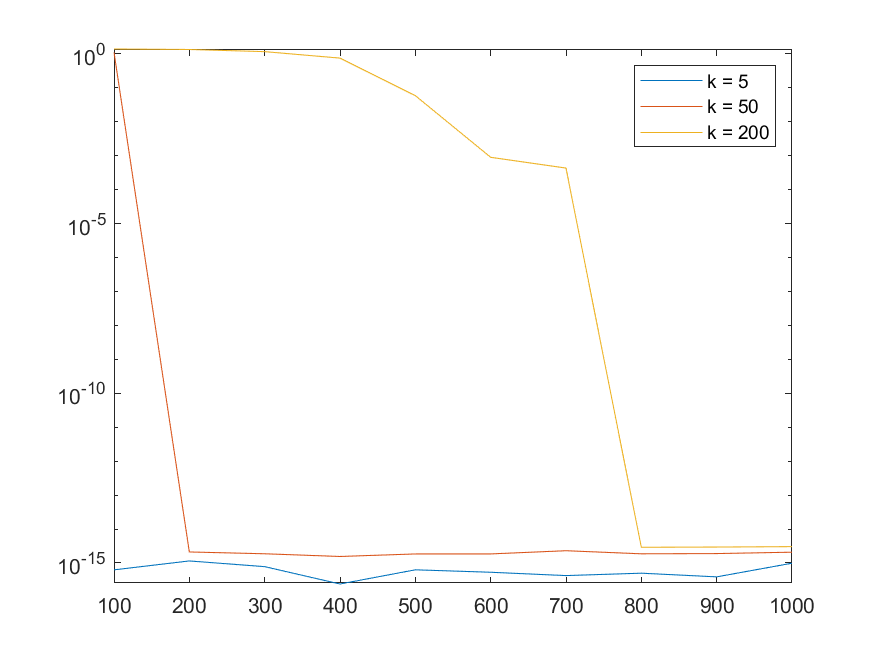
\includegraphics[width=\linewidth]{omp/plot k.png}
        \caption{OMP}
    \end{subfigure}
    \begin{subfigure}{0.45\linewidth}
        \centering
        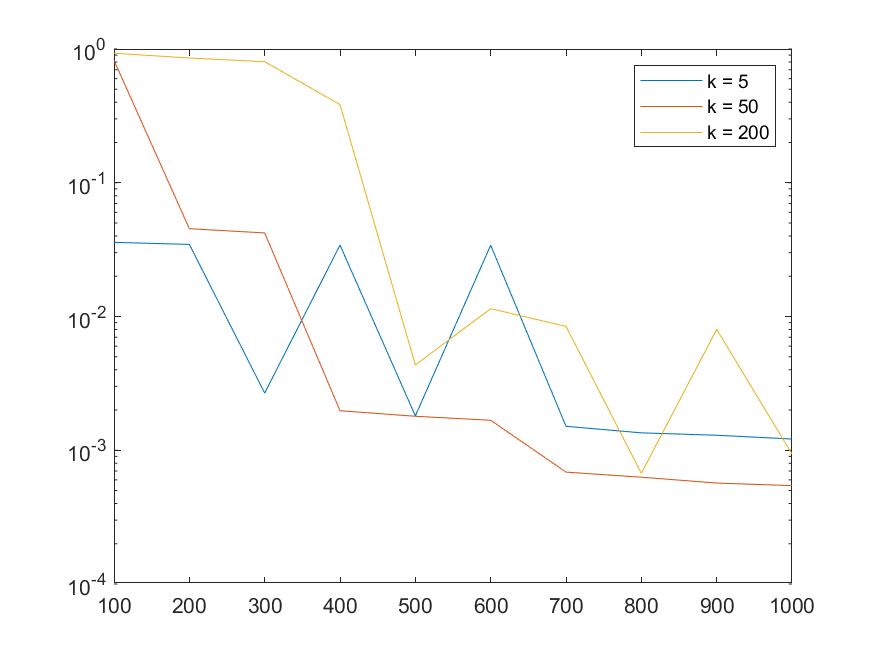
\includegraphics[width=\linewidth]{iht/plot k.png}
        \caption{IHT}
    \end{subfigure}
    \caption{Comparison of OMP and IHT plots for variation with $m$ for a fixed $k$}
    \label{fig:ck}
\end{figure}
\begin{figure}[H]
    \centering
    \begin{subfigure}{0.07\linewidth}
        \centering
        
\includegraphics[width=\linewidth]{omp/k = 5, m = 100.png}
        \caption*{$(5, 100)$}
    \end{subfigure}
    \begin{subfigure}{0.07\linewidth}
        \centering
        
\includegraphics[width=\linewidth]{omp/k = 5, m = 200.png}
        \caption*{$(5, 200)$}
    \end{subfigure}
    \begin{subfigure}{0.07\linewidth}
        \centering
        
\includegraphics[width=\linewidth]{omp/k = 5, m = 300.png}
        \caption*{$(5, 300)$}
    \end{subfigure}
    \begin{subfigure}{0.07\linewidth}
        \centering
        
\includegraphics[width=\linewidth]{omp/k = 5, m = 400.png}
        \caption*{$(5, 400)$}
    \end{subfigure}
    \begin{subfigure}{0.07\linewidth}
        \centering
        
\includegraphics[width=\linewidth]{omp/k = 5, m = 500.png}
        \caption*{$(5, 500)$}
    \end{subfigure}
    \begin{subfigure}{0.07\linewidth}
        \centering
        
\includegraphics[width=\linewidth]{omp/k = 5, m = 600.png}
        \caption*{$(5, 600)$}
    \end{subfigure}
    \begin{subfigure}{0.07\linewidth}
        \centering
        
\includegraphics[width=\linewidth]{omp/k = 5, m = 700.png}
        \caption*{$(5, 700)$}
    \end{subfigure}
    \begin{subfigure}{0.07\linewidth}
        \centering
        
\includegraphics[width=\linewidth]{omp/k = 5, m = 800.png}
        \caption*{$(5, 800)$}
    \end{subfigure}
    \begin{subfigure}{0.07\linewidth}
        \centering
        
\includegraphics[width=\linewidth]{omp/k = 5, m = 900.png}
        \caption*{$(5, 900)$}
    \end{subfigure}
    \begin{subfigure}{0.07\linewidth}
        \centering
        
\includegraphics[width=\linewidth]{omp/k = 5, m = 1000.png}
        \caption*{$(5, 1000)$}
    \end{subfigure}
    \\
    \begin{subfigure}{0.07\linewidth}
        \centering
        
\includegraphics[width=\linewidth]{omp/k = 50, m = 100.png}
        \caption*{$(50, 100)$}
    \end{subfigure}
    \begin{subfigure}{0.07\linewidth}
        \centering
        
\includegraphics[width=\linewidth]{omp/k = 50, m = 200.png}
        \caption*{$(50, 200)$}
    \end{subfigure}
    \begin{subfigure}{0.07\linewidth}
        \centering
        
\includegraphics[width=\linewidth]{omp/k = 50, m = 300.png}
        \caption*{$(50, 300)$}
    \end{subfigure}
    \begin{subfigure}{0.07\linewidth}
        \centering
        
\includegraphics[width=\linewidth]{omp/k = 50, m = 400.png}
        \caption*{$(50, 400)$}
    \end{subfigure}
    \begin{subfigure}{0.07\linewidth}
        \centering
        
\includegraphics[width=\linewidth]{omp/k = 50, m = 500.png}
        \caption*{$(50, 500)$}
    \end{subfigure}
    \begin{subfigure}{0.07\linewidth}
        \centering
        
\includegraphics[width=\linewidth]{omp/k = 50, m = 600.png}
        \caption*{$(50, 600)$}
    \end{subfigure}
    \begin{subfigure}{0.07\linewidth}
        \centering
        
\includegraphics[width=\linewidth]{omp/k = 50, m = 700.png}
        \caption*{$(50, 700)$}
    \end{subfigure}
    \begin{subfigure}{0.07\linewidth}
        \centering
        
\includegraphics[width=\linewidth]{omp/k = 50, m = 800.png}
        \caption*{$(50, 800)$}
    \end{subfigure}
    \begin{subfigure}{0.07\linewidth}
        \centering
        
\includegraphics[width=\linewidth]{omp/k = 50, m = 900.png}
        \caption*{$(50, 900)$}
    \end{subfigure}
    \begin{subfigure}{0.07\linewidth}
        \centering
        
\includegraphics[width=\linewidth]{omp/k = 50, m = 1000.png}
        \caption*{$(50, 1000)$}
    \end{subfigure}
    \\
    \begin{subfigure}{0.07\linewidth}
        \centering
        
\includegraphics[width=\linewidth]{omp/k = 200, m = 100.png}
        \caption*{$(200, 100)$}
    \end{subfigure}
    \begin{subfigure}{0.07\linewidth}
        \centering
        
\includegraphics[width=\linewidth]{omp/k = 200, m = 200.png}
        \caption*{$(200, 200)$}
    \end{subfigure}
    \begin{subfigure}{0.07\linewidth}
        \centering
        
\includegraphics[width=\linewidth]{omp/k = 200, m = 300.png}
        \caption*{$(200, 300)$}
    \end{subfigure}
    \begin{subfigure}{0.07\linewidth}
        \centering
        
\includegraphics[width=\linewidth]{omp/k = 200, m = 400.png}
        \caption*{$(200, 400)$}
    \end{subfigure}
    \begin{subfigure}{0.07\linewidth}
        \centering
        
\includegraphics[width=\linewidth]{omp/k = 200, m = 500.png}
        \caption*{$(200, 500)$}
    \end{subfigure}
    \begin{subfigure}{0.07\linewidth}
        \centering
        
\includegraphics[width=\linewidth]{omp/k = 200, m = 600.png}
        \caption*{$(200, 600)$}
    \end{subfigure}
    \begin{subfigure}{0.07\linewidth}
        \centering
        
\includegraphics[width=\linewidth]{omp/k = 200, m = 700.png}
        \caption*{$(200, 700)$}
    \end{subfigure}
    \begin{subfigure}{0.07\linewidth}
        \centering
        
\includegraphics[width=\linewidth]{omp/k = 200, m = 800.png}
        \caption*{$(200, 800)$}
    \end{subfigure}
    \begin{subfigure}{0.07\linewidth}
        \centering
        
\includegraphics[width=\linewidth]{omp/k = 200, m = 900.png}
        \caption*{$(200, 900)$}
    \end{subfigure}
    \begin{subfigure}{0.07\linewidth}
        \centering
        
\includegraphics[width=\linewidth]{omp/k = 200, m = 1000.png}
        \caption*{$(200, 1000)$}
    \end{subfigure}
    \caption{Each OMP image line is variation with $m$ for a fixed $k$, caption format $(k, m)$}
    \label{fig:ok}
\end{figure}
\begin{figure}[H]
    \centering
    \begin{subfigure}{0.07\linewidth}
        \centering
        
\includegraphics[width=\linewidth]{iht/k = 5, m = 100.png}
        \caption*{$(5, 100)$}
    \end{subfigure}
    \begin{subfigure}{0.07\linewidth}
        \centering
        
\includegraphics[width=\linewidth]{iht/k = 5, m = 200.png}
        \caption*{$(5, 200)$}
    \end{subfigure}
    \begin{subfigure}{0.07\linewidth}
        \centering
        
\includegraphics[width=\linewidth]{iht/k = 5, m = 300.png}
        \caption*{$(5, 300)$}
    \end{subfigure}
    \begin{subfigure}{0.07\linewidth}
        \centering
        
\includegraphics[width=\linewidth]{iht/k = 5, m = 400.png}
        \caption*{$(5, 400)$}
    \end{subfigure}
    \begin{subfigure}{0.07\linewidth}
        \centering
        
\includegraphics[width=\linewidth]{iht/k = 5, m = 500.png}
        \caption*{$(5, 500)$}
    \end{subfigure}
    \begin{subfigure}{0.07\linewidth}
        \centering
        
\includegraphics[width=\linewidth]{iht/k = 5, m = 600.png}
        \caption*{$(5, 600)$}
    \end{subfigure}
    \begin{subfigure}{0.07\linewidth}
        \centering
        
\includegraphics[width=\linewidth]{iht/k = 5, m = 700.png}
        \caption*{$(5, 700)$}
    \end{subfigure}
    \begin{subfigure}{0.07\linewidth}
        \centering
        
\includegraphics[width=\linewidth]{iht/k = 5, m = 800.png}
        \caption*{$(5, 800)$}
    \end{subfigure}
    \begin{subfigure}{0.07\linewidth}
        \centering
        
\includegraphics[width=\linewidth]{iht/k = 5, m = 900.png}
        \caption*{$(5, 900)$}
    \end{subfigure}
    \begin{subfigure}{0.07\linewidth}
        \centering
        
\includegraphics[width=\linewidth]{iht/k = 5, m = 1000.png}
        \caption*{$(5, 1000)$}
    \end{subfigure}
    \\
    \begin{subfigure}{0.07\linewidth}
        \centering
        \includegraphics[width=\linewidth]{iht/k = 50, m = 100.png}
        \caption*{$(50, 100)$}
    \end{subfigure}
    \begin{subfigure}{0.07\linewidth}
        \centering
        \includegraphics[width=\linewidth]{iht/k = 50, m = 200.png}
        \caption*{$(50, 200)$}
    \end{subfigure}
    \begin{subfigure}{0.07\linewidth}
        \centering
        \includegraphics[width=\linewidth]{iht/k = 50, m = 300.png}
        \caption*{$(50, 300)$}
    \end{subfigure}
    \begin{subfigure}{0.07\linewidth}
        \centering
        \includegraphics[width=\linewidth]{iht/k = 50, m = 400.png}
        \caption*{$(50, 400)$}
    \end{subfigure}
    \begin{subfigure}{0.07\linewidth}
        \centering
        \includegraphics[width=\linewidth]{iht/k = 50, m = 500.png}
        \caption*{$(50, 500)$}
    \end{subfigure}
    \begin{subfigure}{0.07\linewidth}
        \centering
        \includegraphics[width=\linewidth]{iht/k = 50, m = 600.png}
        \caption*{$(50, 600)$}
    \end{subfigure}
    \begin{subfigure}{0.07\linewidth}
        \centering
        \includegraphics[width=\linewidth]{iht/k = 50, m = 700.png}
        \caption*{$(50, 700)$}
    \end{subfigure}
    \begin{subfigure}{0.07\linewidth}
        \centering
        \includegraphics[width=\linewidth]{iht/k = 50, m = 800.png}
        \caption*{$(50, 800)$}
    \end{subfigure}
    \begin{subfigure}{0.07\linewidth}
        \centering
        \includegraphics[width=\linewidth]{iht/k = 50, m = 900.png}
        \caption*{$(50, 900)$}
    \end{subfigure}
    \begin{subfigure}{0.07\linewidth}
        \centering
        \includegraphics[width=\linewidth]{iht/k = 50, m = 1000.png}
        \caption*{$(50, 1000)$}
    \end{subfigure}
    \\
    \begin{subfigure}{0.07\linewidth}
        \centering
        \includegraphics[width=\linewidth]{iht/k = 200, m = 100.png}
        \caption*{$(200, 100)$}
    \end{subfigure}
    \begin{subfigure}{0.07\linewidth}
        \centering
        \includegraphics[width=\linewidth]{iht/k = 200, m = 200.png}
        \caption*{$(200, 200)$}
    \end{subfigure}
    \begin{subfigure}{0.07\linewidth}
        \centering
        \includegraphics[width=\linewidth]{iht/k = 200, m = 300.png}
        \caption*{$(200, 300)$}
    \end{subfigure}
    \begin{subfigure}{0.07\linewidth}
        \centering
        \includegraphics[width=\linewidth]{iht/k = 200, m = 400.png}
        \caption*{$(200, 400)$}
    \end{subfigure}
    \begin{subfigure}{0.07\linewidth}
        \centering
        \includegraphics[width=\linewidth]{iht/k = 200, m = 500.png}
        \caption*{$(200, 500)$}
    \end{subfigure}
    \begin{subfigure}{0.07\linewidth}
        \centering
        \includegraphics[width=\linewidth]{iht/k = 200, m = 600.png}
        \caption*{$(200, 600)$}
    \end{subfigure}
    \begin{subfigure}{0.07\linewidth}
        \centering
        \includegraphics[width=\linewidth]{iht/k = 200, m = 700.png}
        \caption*{$(200, 700)$}
    \end{subfigure}
    \begin{subfigure}{0.07\linewidth}
        \centering
        \includegraphics[width=\linewidth]{iht/k = 200, m = 800.png}
        \caption*{$(200, 800)$}
    \end{subfigure}
    \begin{subfigure}{0.07\linewidth}
        \centering
        \includegraphics[width=\linewidth]{iht/k = 200, m = 900.png}
        \caption*{$(200, 900)$}
    \end{subfigure}
    \begin{subfigure}{0.07\linewidth}
        \centering
        \includegraphics[width=\linewidth]{iht/k = 200, m = 1000.png}
        \caption*{$(200, 1000)$}
    \end{subfigure}
    \caption{Each IHT image line is variation with $m$ for a fixed $k$, caption format $(k, m)$}
    \label{fig:ik}
\end{figure}
\subsection{Task 3}
For $m \in \{500,700\}$ and $k \in \{5,10,20,30,50,100,150,200\}$.

RMSE plots are shown in \ref{fig:cm} and reconstructed images are shown in \ref{fig:om} and \ref{fig:im}.

Reconstructed images are very similar to the original images and the RMSE plots indicates (with some exceptions) that for higher $m$, higher $k$ (sparsity) can be handled before the RMSE increases.
\begin{figure}[H]
    \centering
    \begin{subfigure}{0.45\linewidth}
        \centering
        \includegraphics[width=\linewidth]{omp/plot m.png}
        \caption{OMP}
    \end{subfigure}
    \begin{subfigure}{0.45\linewidth}
        \centering
        \includegraphics[width=\linewidth]{iht/plot m.png}
        \caption{IHT}
    \end{subfigure}
    \caption{Comparison of OMP and IHT plots for variation with $k$ for a fixed $m$}
    \label{fig:cm}
\end{figure}
\begin{figure}[H]
    \centering
    \begin{subfigure}{0.12\linewidth}
        \centering
        \includegraphics[width=\linewidth]{omp/k = 5, m = 500.png}
        \caption{$(5, 500)$}
    \end{subfigure}
    \begin{subfigure}{0.12\linewidth}
        \centering
        \includegraphics[width=\linewidth]{omp/k = 10, m = 500.png}
        \caption{$(10, 500)$}
    \end{subfigure}
    \begin{subfigure}{0.12\linewidth}
        \centering
        \includegraphics[width=\linewidth]{omp/k = 20, m = 500.png}
        \caption{$(20, 500)$}
    \end{subfigure}
    \begin{subfigure}{0.12\linewidth}
        \centering
        \includegraphics[width=\linewidth]{omp/k = 30, m = 500.png}
        \caption{$(30, 500)$}
    \end{subfigure}
    \begin{subfigure}{0.12\linewidth}
        \centering
        \includegraphics[width=\linewidth]{omp/k = 50, m = 500.png}
        \caption{$(50, 500)$}
    \end{subfigure}
    \begin{subfigure}{0.12\linewidth}
        \centering
        \includegraphics[width=\linewidth]{omp/k = 100, m = 500.png}
        \caption{$(100, 500)$}
    \end{subfigure}
    \begin{subfigure}{0.12\linewidth}
        \centering
        \includegraphics[width=\linewidth]{omp/k = 150, m = 500.png}
        \caption{$(150, 500)$}
    \end{subfigure}
    \begin{subfigure}{0.12\linewidth}
        \centering
        \includegraphics[width=\linewidth]{omp/k = 200, m = 500.png}
        \caption{$(200, 500)$}
    \end{subfigure}
    \begin{subfigure}{0.12\linewidth}
        \centering
        \includegraphics[width=\linewidth]{omp/k = 5, m = 700.png}
        \caption{$(5, 700)$}
    \end{subfigure}
    \begin{subfigure}{0.12\linewidth}
        \centering
        \includegraphics[width=\linewidth]{omp/k = 10, m = 700.png}
        \caption{$(10, 700)$}
    \end{subfigure}
    \begin{subfigure}{0.12\linewidth}
        \centering
        \includegraphics[width=\linewidth]{omp/k = 20, m = 700.png}
        \caption{$(20, 700)$}
    \end{subfigure}
    \begin{subfigure}{0.12\linewidth}
        \centering
        \includegraphics[width=\linewidth]{omp/k = 30, m = 700.png}
        \caption{$(30, 700)$}
    \end{subfigure}
    \begin{subfigure}{0.12\linewidth}
        \centering
        \includegraphics[width=\linewidth]{omp/k = 50, m = 700.png}
        \caption{$(50, 700)$}
    \end{subfigure}
    \begin{subfigure}{0.12\linewidth}
        \centering
        \includegraphics[width=\linewidth]{omp/k = 100, m = 700.png}
        \caption{$(100, 700)$}
    \end{subfigure}
    \begin{subfigure}{0.12\linewidth}
        \centering
        \includegraphics[width=\linewidth]{omp/k = 150, m = 700.png}
        \caption{$(150, 700)$}
    \end{subfigure}
    \begin{subfigure}{0.12\linewidth}
        \centering
        \includegraphics[width=\linewidth]{omp/k = 200, m = 700.png}
        \caption{$(200, 700)$}
    \end{subfigure}
    \caption{Each OMP image line is variation with $k$ for a fixed $m$, caption format $(k, m)$}
    \label{fig:om}
\end{figure}
\begin{figure}[H]
    \centering
    \begin{subfigure}{0.12\linewidth}
        \centering
        \includegraphics[width=\linewidth]{iht/k = 5, m = 500.png}
        \caption{$(5, 500)$}
    \end{subfigure}
    \begin{subfigure}{0.12\linewidth}
        \centering
        \includegraphics[width=\linewidth]{iht/k = 10, m = 500.png}
        \caption{$(10, 500)$}
    \end{subfigure}
    \begin{subfigure}{0.12\linewidth}
        \centering
        \includegraphics[width=\linewidth]{iht/k = 20, m = 500.png}
        \caption{$(20, 500)$}
    \end{subfigure}
    \begin{subfigure}{0.12\linewidth}
        \centering
        \includegraphics[width=\linewidth]{iht/k = 30, m = 500.png}
        \caption{$(30, 500)$}
    \end{subfigure}
    \begin{subfigure}{0.12\linewidth}
        \centering
        \includegraphics[width=\linewidth]{iht/k = 50, m = 500.png}
        \caption{$(50, 500)$}
    \end{subfigure}
    \begin{subfigure}{0.12\linewidth}
        \centering
        \includegraphics[width=\linewidth]{iht/k = 100, m = 500.png}
        \caption{$(100, 500)$}
    \end{subfigure}
    \begin{subfigure}{0.12\linewidth}
        \centering
        \includegraphics[width=\linewidth]{iht/k = 150, m = 500.png}
        \caption{$(150, 500)$}
    \end{subfigure}
    \begin{subfigure}{0.12\linewidth}
        \centering
        \includegraphics[width=\linewidth]{iht/k = 200, m = 500.png}
        \caption{$(200, 500)$}
    \end{subfigure}
    \begin{subfigure}{0.12\linewidth}
        \centering
        \includegraphics[width=\linewidth]{iht/k = 5, m = 700.png}
        \caption{$(5, 700)$}
    \end{subfigure}
    \begin{subfigure}{0.12\linewidth}
        \centering
        \includegraphics[width=\linewidth]{iht/k = 10, m = 700.png}
        \caption{$(10, 700)$}
    \end{subfigure}
    \begin{subfigure}{0.12\linewidth}
        \centering
        \includegraphics[width=\linewidth]{iht/k = 20, m = 700.png}
        \caption{$(20, 700)$}
    \end{subfigure}
    \begin{subfigure}{0.12\linewidth}
        \centering
        \includegraphics[width=\linewidth]{iht/k = 30, m = 700.png}
        \caption{$(30, 700)$}
    \end{subfigure}
    \begin{subfigure}{0.12\linewidth}
        \centering
        \includegraphics[width=\linewidth]{iht/k = 50, m = 700.png}
        \caption{$(50, 700)$}
    \end{subfigure}
    \begin{subfigure}{0.12\linewidth}
        \centering
        \includegraphics[width=\linewidth]{iht/k = 100, m = 700.png}
        \caption{$(100, 700)$}
    \end{subfigure}
    \begin{subfigure}{0.12\linewidth}
        \centering
        \includegraphics[width=\linewidth]{iht/k = 150, m = 700.png}
        \caption{$(150, 700)$}
    \end{subfigure}
    \begin{subfigure}{0.12\linewidth}
        \centering
        \includegraphics[width=\linewidth]{iht/k = 200, m = 700.png}
        \caption{$(200, 700)$}
    \end{subfigure}
    \caption{Each IHT image line is variation with $k$ for a fixed $m$, caption format $(k, m)$}
    \label{fig:im}
\end{figure}
\end{document}